\documentclass{beamer}

\usepackage{mathtools}                  % Use amsmath + fixes
\usepackage{amssymb}                    % More mathematical symbols
\usepackage{siunitx}                    % Correctly formatted units
\usepackage{physics}                    % More notation
\usepackage{nicefrac}
\usepackage{xfrac}
\usepackage{listings}

%%%%%  NOMENCLATURE  %%%%%
\usepackage{acro}                       % Expand, list, and link acronyms

%%%%%  FIGURES  %%%%%
\usepackage{import}
\usepackage{graphicx}                   % Include images
\usepackage{pdfpages}                   % Include PDFs
\usepackage{standalone}

\usepackage{tikz}


\title{Concurrent Marked Graph Execution on Single-Thread Processors}
\author{Sam Spekreijse}
\date{02/10/2020}



\begin{document}
	\begin{frame}%[plain]
	\titlepage
	\end{frame}


	\begin{frame}
	\frametitle{Marked Graphs}
	Marked graphs are directed graphs with alternating nodes of two types. 
	These two types represent states and transitions. 

	\vspace{1cm}

	Similar to normal directed graphs, marked graphs can be stored in several ways. 
	The two most common are:
		\begin{itemize}
		\item Adjacency List: Each vertex stores a list of edges. 
		\item Adjacency Matrix: A lookup table for a given start and end node. 
		\end{itemize}
	\end{frame}


	\begin{frame}
	\frametitle{Wikipedia's Basic Example}
	\includegraphics[width=1.0\textwidth]{Marked_Graph_example1.png}
	\end{frame}


	\begin{frame}
	\frametitle{A More Interesting Example}
	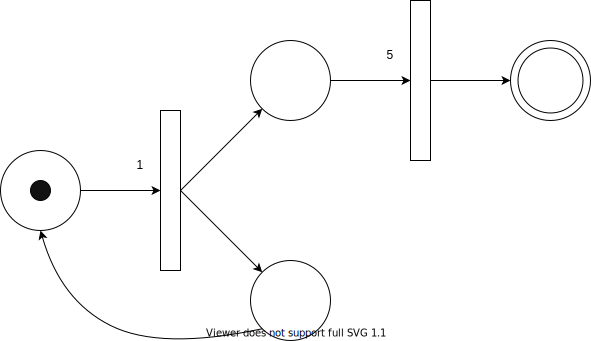
\includegraphics[width=1.0\textwidth]{loop.png}
	\end{frame}


	\begin{frame}
	\frametitle{Priority Properties}
	Priorities should be inherited from the `parent' process every time a process forks. 

	\vspace{1cm}

	How to store the priorities is therefore not straightforward. 
	Both string-based and float-based systems were considered. 
	At present, a linked list is used, and the priority of each process is not explicitly known. 
	\end{frame}


	\begin{frame}[fragile]
	\frametitle{Implementation}
		\begin{lstlisting}[language=c]
typedef struct Fsm_s Fsm_t;
typedef struct FsmState_s FsmState_t;
typedef int32_t FsmTransId_t;
typedef FsmTransId_t *(FsmFunc_t)(void);


typedef struct {
	bool isLockstep;
	size_t numProcesses; 

	size_t numInProcesses;
	Process_t **processes; 
	size_t numOutProcesses;
	FsmState_t **outStates; 
} FsmTrans_t;

		\end{lstlisting}


	\end{frame}


	\begin{frame}[fragile]
		\begin{lstlisting}
struct FsmState_s{
	//One of the following must be NULL. 
	Fsm_t *subFsm;
	FsmFunc_t *func;
	
	size_t numTransitions;
	FsmTrans_t **transitions;
};


struct Fsm_s {
	Fsm_t *parent;
	FsmState_t *end;
	size_t numStates;
	FsmState_t *states[]; 
};

		\end{lstlisting}
	\end{frame}


	\begin{frame}[fragile]
		\begin{lstlisting}
typedef struct process_s Process_t;
typedef struct process_s {
	bool isActive;
	FsmState_t *state;

	Process_t *prev;
	Process_t *next;
};

		\end{lstlisting}
	\end{frame}


	\begin{frame}
	\frametitle{Additional Developments}
	Recursive UML statecharts support, where states can themselves also be FSMs, was also part of this project. 
	This functionality can be implemented via FSM expansion at compile time, or by changing the runtime. 
	The latter option has been implemented for debugging purposes. 

	\vspace{1cm}

	The nature of marked graphs is that each transition can be used not only to synchronise processes, but to synchronise processors operating in lockstep. 
	Each transition has the option of being a synchronising transition. 
	This enables modular redundancy to be designed into the application from the first planning stages. 
	\end{frame}

\end{document}

